\section{Architecture of distributed systems}

This section introduces and analyzes common design patterns of distributed
systems. It is divided into two subsections based on
CAP-theorem\cite{gilbert2002brewer} that states that no distributed system can
achieve consistency, availability and partition tolerance at the same time. Due
the nature of distributed systems network partitions are bound to happen, thus
designers of distributed system need to choose whether the system remains
available during the partition or keeps the data consistent.

\subsection{CP-systems}

\begin{figure}[h!]
  \centering
    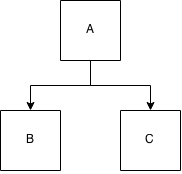
\includegraphics{pictures/cp_system.png}
  \caption{CP-system with a single master node and two slaves}
\label{cpimage}
\end{figure}

CP-systems endorse data consistency over availability. In practice this means
that when a network between two or more database nodes malfunctions, the
system should stop handling both, read and write requests from clients and wait
until the network is healed. Failure to do so might bring the systems into an
inconsistent state, where nodes of the system have different view of the same
datum. Consider figure~\ref{cpimage} that shows a CP-system consisting of a
single master node \(A\) and two slaves \(B\) and \(C\). Clients are able to
read from all of the nodes, but only node \(A\) accepts writes. After a
successful write, \(A\) replicates the write to the slave nodes. If the
connection between \(A\) and \(B\) fails, the system is partitioned into two
sets, one containing \(A\) and \(C\), and other containing only \(B\). Now if
the client first writes a new document to \(A\) and then tries to read it from
both \(B\) and \(C\), what happens is that \(C\) correctly returns the written
document, but \(B\) reports that the document can not be found. This happens
because master \(A\) was not able to replicate the new write to node \(B\)
because the network between the nodes was down. Because now \(B\) and \(C\) have
a different view of the same datum, the system can not be considered as
CP-system anymore. The situation can be fixed by not accepting a write from the
client, when the master node detects that it is not able to replicate the writes
to all nodes. 

As in the example, a common way to model CP-systems is a master/slave
architecture, where one node at a time acts as a master and other nodes are
slaves. To achieve consistency, only master is able to accept write requests and
depending on the architecture, slaves might be able to accept read requests. If
slaves handle the read requests, the distributed system might not be consistent
at all times. For example, node \(A\) accepted a write but did not had time to
replicate it to node \(B\) when it replies to the read request accessing that
object, the database would incorrectly report that object is not found. However
after \(A\) has replicated the object to \(B\) the database is again in
consistent state. This is called eventual consistency.

Vogels specifies eventual consistency as a specific form of weak
consistency\cite{vogels2009eventually}. A system with weak consistency does not
guarantee that subsequent accesses to the updated object always returns the
updated object but a set of conditions need to be met before. The period between
when the object is updated and when it is guaranteed is called
\emph{inconsistency window}.

In eventual consistency, the system guarantees that if no new updates are made
to the object, eventually all access will return the updated object. In this
case, the maximum inconsistency window in best case scenario can be calculated
from different factors of the system, such as communication delay between nodes
and the load of the system. Of course in exceptional events such as network
partition the inconsistency window can grow as large as the event occur.

The problem that many CP-systems face is what happens when the master node
becomes unavailable. That may occur for many reasons, for example the node can
suffer from hardware failure or the network between master and other nodes goes
down. Naturally the system needs to be able to recover from such cases and many
different procedures have been developed to cope with the problem. Next we
discuss how Raft consensus algorithm handles election of a new leader.

Raft is a consensus algorithm developed to replace more complex algorithm Paxos.
Raft aims to be more understandable and better uncoupled than its
predecessor\cite{chiefari1998living}. Consensus algorithms allow collection of
services to agree on some state even when some of them fails. They often arise
in context of \emph{replicated state machines}, where each service compute
identical copies of the same data. To achieve consistency, Raft selects a
distinguished leader which has a complete responsibility of managing the
replicated log and replicating them to other services. When the leader fails or
becomes unavailable, the new leader must be elected.

Raft detects leader failures with heartbeats. Each node starts as a follower and
remains in that state as long as it receives heartbeat signals from the leader.
If a follower receives no heartbeat in a period of time called \emph{election
timeout}, it assumes there are no leader and begins the leader election.

In the beginning of leader election, the follower that received no heartbeat
promotes itself to a candidate and sends vote request messages to the other
clients. A client grants the vote for the first candidate requesting the vote
and declines the rest. The candidate continues in this state until one of the
three things things happens:

\begin{enumerate}
  \item The candidate wins the election and promotes itself to the leader if it
  receives votes from majority of the cluster. Once the candidate wins the
  election it starts sending heartbeats to the other nodes and establishes the
  authority and prevents new elections.
  \item While waiting for the votes, the candidate might receive a heartbeat
  from other node. In this case it demotes itself to the follower state and
  recognizes the new leader.
  \item Last outcome is that the candidate does not win or lose the elections.
  If many followers become candidates at the same time, it is possible that none
  of the candidates receive majority of votes and initiate a new round of
  vote requests. Raft uses randomized election time outs to ensure that no two
  clients are candidates indefinitely. Another candidate might still be waiting
  out the time out when other candidate receives a majority of the votes and
  starts sending heartbeats and ending elections.
\end{enumerate}

The actual leader election in RAFT is a bit more complicated than described
above, having a concept of \emph{terms} to measure time as a logical clocks, but
they were left out for clarity. The original paper explains the election in more
detail and the website of Raft
algorithm\footnote{\url{https://raftconsensus.github.io/}} has an excellent
interactive visualization about the leader election.

\subsection{AP-systems}

\begin{figure}[h!]
  \centering
    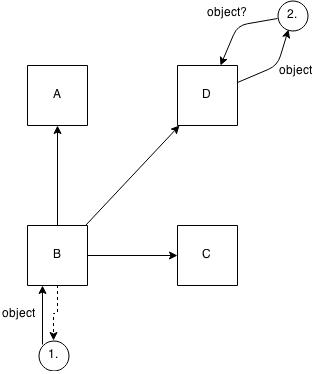
\includegraphics[scale=0.7]{pictures/ap_system.png}
  \caption{AP-system where client 1.\ sends a write request which is replicated
  to all the nodes and is read afterwards by client 2.}
\label{apimage}
\end{figure}

AP-systems choose to be available in the event of network partition instead of
keeping the data consistent at all times. In practice this means that all nodes
of the cluster are allowed to handle both read and writes requests from clients
and there is no dedicated master node. After receiving the request, the
node can either handle the request itself or delegate it to more appropriate
node for processing. Depending from the architecture, the write may be
acknowledged when the handling node has received it, or it might require
acknowledges from multiple nodes. After a successful write of an object, the
object is replicated to other nodes for a better durability and availability.
Even if a node that originally handled the write request is unavailable, the
cluster is able to respond to the request.

Figure~\ref{apimage} shows an AP-system with four nodes and two clients. First
client \(1\) sends a write request to the node \(B\) which acknowledges it
immediately, displayed as a dashed line. It then replicates the object to the
other nodes. Later client \(2\) sends a read request for the same object that
can be handled by \(D\) since it has received the object. Next consider a case
where the network is split into two different groups, client \(1\) and nodes
\(A\) and \(B\) belong to the first group and client \(2\) and nodes \(C\) and
\(D\) to second.

Because AP-systems promote availability over consistency, the system should be
able to accept writes even if the network in the cluster is malfunctioning. In
the situation of the example but with a partitioned network, client \(1\) had
sent the write request, and the write would have been acknowledged normally.
However \(B\) would have been unable to replicate the object to the nodes in the
other side of the partition and client \(2\) had got \texttt{not\_found}
response from node \(D\). This shows an important characteristics of AP-systems,
because consistency is sacrificed to obtain better availability, the service
might get into an inconsistent state but still return successful response codes
to the user. In contrast, CP-system would have rejected the write request from
\(1\) because it could not reach other nodes thus making the system unavailable.

Another interesting problem arises when a network partition heals. Assume that
both sides of the partition have received an update to the same object. Because
AP-systems do not require the write is acknowledged by majority of nodes, both
sides might end up with its own version of the same object. When the network
heals, both sides try to replicate their version to the other side but run into
a problem. Which version is correct?

Some systems solve the problem by tracking the time when an update was received
and then choosing an object with higher timestamp. This solves the problem, but
effectively destroys updates received by the other object. The system might keep
the discarded version safe so the user can try to manually merge the two
versions later. It might be tempting to try to write an universal merge function
that merges the changes from both objects in all cases. However it can be shown
that such function does not exists\todo{how is this done?}.

Because it is impossible for the AP-system to recover from all conflict cases, a
careful thought should be placed on the conflict detection. Although concurrent
updates by different clients always end up in conflict, it is possible to
automatically solve serializable updates if detected correctly. A naive way to
detect a conflict between two versions is to compare the hashes of the versions
and check whether they differ. However this approach might lead into a false
positives that can be eliminated.

TODO: Example, client 1 creates an object and after replication a network
partition occurs. Now client 1 updates ``left'' side once. Then client 2 reads
an updated document from ``left'' side and updates it to the ``right'' side.
Because the history is serializable we should be able to merge the history
automatically, (first a write from 1, then write from 2), but when comparing
only hash we don't know that. Vector clocks solve the issue. (Assign a clock for
both clients, and then on the merge the ``right'' side knows it has a ascendant
of the ``left'' side's version). Serve with nice images.
